\chapter{AWS Implementation of Reinforcement Learning}
Author: Florian Schwarzl

With DeepRacer, Amazon has created their own implementation of reinforcement learning, geared towards developers, with focus on learning about machine learning concepts. Compared to other robotics competitions, the DeepRacer League is more proprietary, as it is not just intended as a way of leaning about Machine Learning, but also a way for Amazon to promote its services. As a result, Amazon has tailored the reinforcement learning environment to suit their services. 

\section{Concept}
Reinforcement learning as a whole is a complex topic that can seem overwhelming. In order to simplify the learning process and create an even playing field for all participants, only some parts of the entire learning process can be modified. When training via the AWS cloud, Amazon allows only the configuration of certain hyperparameters, the action space and the creation of a custom reward function. This reward function, whose purpose was explained earlier, represents the core of their implementation. It has by far the largest impact on the performance of the car both in simulations and real world scenarios. Apart from those two modifications, Amazon offers very little in terms of customisation. This simplification has multiple reasons, the first one being that, as mentioned earlier, it offers programmers with less experience in reinforcement learning the option to participate in the races. Amazon themselves label the DeepRacer as a way to learn about machine learning.The second reason behind this simplification is that it provides a common basis for the races, which, like in any sport, is required in order to provide a fair competition.

\section{Training architecture}

\section{Reward Function}
The reward function determines the reward the agent receives for taking a certain action. Therefor the reward has to depend on the environment and the situation in which the agent is currently in, which is called the state. As it is not possible to capture all aspects of a situation, the actual state is abstracted into a predefined set of parameters. These parameters are the foundation which the entire reward process is based upon. 

The function itself is written in python and has to return a floating point number, which will from here on be called reward. The reward represents the immediate feedback the agent receives when moving along the track. This feedback acts as an incentive plan an what action the agent will take. If an incentive plan is not considered carefully, it can lead to unintended consequences of opposite effect. This is the case because an immediate reward alone is not enough to determine if an action has a positive effect, as this affect can come up delayed. This requires not only the current action but also subsequent actions to earn a positive reward for the agent in order for it to consider the initial action preferable.\repeatfootcite[][p. 31 f.]{AWS19} 


One example of such unintended consequences of opposite effect occurred during one of the first training sessions. Using a simple reward function which took only the speed and offset from the centre line into consideration, the agent began to drive in a zig-zag pattern on the centre line. The reason behind this was that the reward function gave a significant reward for staying close to the centre of the track. Following this concept, the agent maximised the received reward by diving in said pattern. However due to this behaviour the vehicle performed poorly in terms of speed and was prone to going off track, especially when tested on a physical track in a real world environment. Avoiding scenarios like the one described above is crucial to creating and training functioning models.

\subsection{Parameter Reference}
The reward function receives a predetermined set of parameters, supplied via a Python dictionary. These parameters represent the abstracted information available to the agent during  training and, subsequently, during testing. They are abstracted from the image provided by the single camera. This abstraction causes a natural loss in accuracy, as it is neither feasible nor possible to capture a complete picture of the environment in which the agent takes its actions. Taking into account this gap in precision and modifying training behaviour accordingly  represents a major part in creating working models.

Not every parameter given has to be used in order for the reward function to be usable. Simpler functions might only rely on the speed and distance to the centre line and still manage to consistently complete laps. The following subsections represent a list parameters which we used in our reward functions, in the order in which we first made use of them. Reference is taken from the official DeepRacer documentation.\repeatfootcite[][p. 59 ff.]{AWS19}

\subsubsection{Parameter: track width}
This parameter is one of the simplest, yet also one of the most important. It represents the width of the current track in meters as a float value. The width of the track is used to give other parameters, like the distance between the car and the centre line enough context to be useful. Without this reference, the relative position of the vehicle on the track can not be determined. This is why this parameter is often used in tandem with the distance from the centre line, as described in the following subsection.

\subsubsection{Parameter: distance from centre}
Similar to the previous parameter, this one is used primarily to determine the relative position of the car on the track. Combining these values, the track width and the distance from the centre line, is sufficient for creating a simple reward function that will teach the model to follow the centre line. The following code listing shows a basic reward function utilising these two parameters. The track is divided into three sections on either side of the centre line. The reward is based on the sections, with those further away from the centre giving less reward.
% maybe write more

\begin{minipage}{\linewidth}
\begin{lstlisting}[language={Python},label={lst:reward_distance}, caption={Reward function using track width and distance from centre}]
def reward_function(params):

    track_width = params['track_width']
    distance_from_center = params['distance_from_center']

    marker_10_percent = 0.1 * track_width
    marker_25_percent = 0.25 * track_width
    marker_50_percent = 0.5 * track_width

    if distance_from_center <= marker_10_percent:
        reward = 1.0
    elif distance_from_center <= marker_25_percent:
        reward = 0.5
    elif distance_from_center <=marker_50_percent:
        reward = 0.1
    else:
        reward = 1e-3

    return float(reward)
\end{lstlisting}
\end{minipage}

\subsubsection{Parameter: speed}
This parameter contains the current speed of the agent in metres per second. The float value ranges from 5 metres per second, the top speed of the car, to 0 metres per second. It is important to note that this parameter is the absolute velocity, meaning all values will be greater or equal to 0, even when going backwards. Although this is one of, if not the simplest parameter provided, it is non the less one of the most important values. After all, the concept of the DeepRacer project is to race cars controlled solely by machine learning algorithms. Therefor speed is in the end the deciding factor. One might think that the usage of this parameter is simple, increase the reward the agent receives when it is driving faster. This will definitely lead to the agent going fast, too fast in fact. 

As it is in the real world, driving through a turn at high speed might result in the car losing contact with the road and subsequently going off said road. Most notably during the early stages of training, the agent was incited to drive at a slower, more constant speed. By default, the agent tries to move as fast as possible, which inevitably leads to the car going off track during testing on real tracks. Keeping this default behaviour in mind, performance will increase notably during early training sessions if the agent receives a reward for staying at a medium speed rather than going full throttle.

%
% TODO: Empfohlene Werte aus  Training Sessions
%

\subsubsection{Parameter: steps}
The step parameter, or rather the step count is an integer which count the action taken by the agent during a lap. As said, one step corresponds to one action taken by the agent according to the current policy. This parameter might not seem like an important value to consider, but depending on the reward function used, it is essential to creating a model capable of driving on a real-world track.
Let us take the reward function displayed in \ref{lst:reward_distance} as an example. In this the agent receives an increased reward for staying near the centre line. In order to achieve this, the agent corrects its movement should it divert too much from the line. This diversion can be caused my several things, for example an uneven track, different traction on the wheels or simply by inaccuracy when steering, all of which can occur frequently in a real world scenario. In the simulated environment however, such discrepancies have to be manually inserted, as seen in Section \ref{sec:BackgroundNoise}. Without the manually added noise, the agent will learn to constantly correct its movement, staying as close to the middle as possible. Such a behaviour could be observed during our first training sessions. A model trained this way will perform poorly during testing on real tracks, since it is permanently trying to steer.

Penalising the agent for taking far more steps than required is one way to prevent it from driving in a zig-zag pattern.

\subsubsection{Parameter: Coordinates x, y}
Although this pair of parameters is rarely used in the reward function, the coordinate system is useful to know if other parameters, namely the waypoints, want to be used. This parameter provides a list of tuples, which contain a pair of coordinates. These coordinates describe the current position of the vehicle relative to the bottom left corner of the simulated world. It is important to note that the point of origin is not the border of the track but rather the border of the predefined, simulated world. Taking this into consideration, it is questionable how accurately these coordinates will be when used during deployment on a real track.

\subsubsection{Parameter: waypoints}\label{sec:param_waypoints}
This parameter is, together with others related to the waypoint system, one of the option for navigating along the track. Each simulation world has a predefined set of waypoints distributed along the centre line of the track. These waypoints or markers are stored in this parameter, which is a list of tuples. Every tuple represents a single waypoint in the form of its coordinates along the x-axis and y-axis, respectively. The frequency and total number of waypoints differs greatly between tracks. More so, there is no official documentation about where these are located along the track. Most tracks have three sets of markers. The first line is located at the outer border, the second one is on the middle line and the third represents the inner track limit. The waypoints can be found in NumPy-files, stored in a two-dimensional array containing tuples. The inner array contains three points in total. The first point is the one on the outer border, the second one is in the middle and the third one is located on the inside.

\subsubsection{Waypoint visualisation}
As stated in the previous section, Amazon provides no information on where the waypoints of a given track are located. The only information given is via the parameters supplied to the reward function and a set of NumPy-files. These files hold a multidimensional array containing the coordinates of all markers on a certain track. The files can be found in official AWS repositories meant for workshops with the DeepRacer.\footnote{https://github.com/aws-samples/aws-deepracer-workshops} The files contain all waypoints in binary format. They can be accessed easily using the python library NumPy.\repeatfootcite{numpy}
The same package has been used by the ARCC\footnote{Autonomous Race Car Community} to provide a simple Python program which creates a plot using the coordinates from the file. This plot can then be viewed and saved, providing a precise visualisation of all waypoints on a track. The python script itself is simple. This offers the possibility for improvement, for example an option to provide the track name as an parameter when executing the script, rather than changing the name in the source code.

\begin{figure}
    \centering
    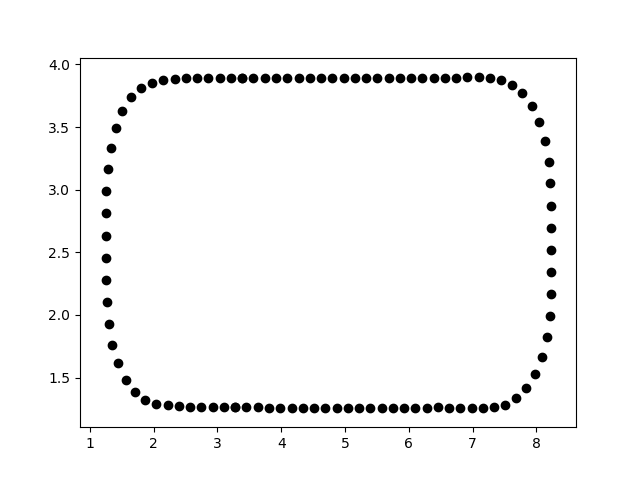
\includegraphics[width=.85\textwidth]{images/oval_track_waypoints2.png}
    \caption{Waypoints of oval track}
    \label{fig:waypoints_oval}
\end{figure}

The figure \ref{fig:waypoints_oval} shows all waypoints of the oval track according to the coordinates they are associated with. It should be noted that on the short sides of the oval there are fewer waypoints per unit of length as on the long sides. This figure also demonstrates the system of coordinates stretched across each simulated world and how these coordinates relate to the real world. Most notably, that the point of origin is in fact not the bottom left corner of the road but rather the bottom left corner of the simulation. Figure \ref{fig:waypoints_oval_all} visualises all markers located on this track.

\begin{figure}
    \centering
    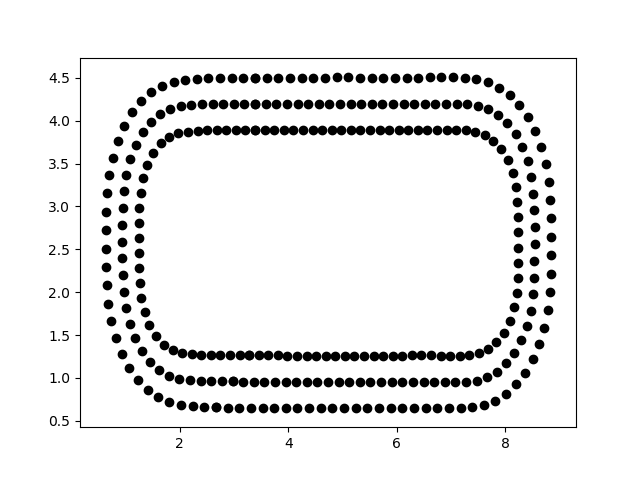
\includegraphics[width=.85\textwidth]{images/oval_track_waypoints_all.png}
    \caption{All waypoints of oval track}
    \label{fig:waypoints_oval_all}
\end{figure}

\subsubsection{Parameter: closest waypoints}
Waypoints and their purpose have already been covered in the previous two section. This section completes the set of parameters regarding waypoints. This parameter provides a list containing the indices of the two waypoints closest to the agent at the current moment. These indices refer to the waypoint for the list of waypoints, discussed in section \ref{sec:param_waypoints}. Combining this information with the heading and coordinates of the agent, it is possible to create a reward function based entirely on these milestones. It is not clear however which waypoint is returned. It could be that only the centre line of markers is used in this function or that the ones located at the track limits are used as well. In this regard, the official documentation is lacking precise information.

\section{Action Space}
This section covers all aspects regarding the action space.
\subsection{Definition}
The action space of the agent, that being the car, describes, what it can do. It specifies a finite set of action from which the agent can choose during training. An action is defined by two dimensions, speed and steering angle. The number of actions as well as the granularity between them can be altered as needed. In the context of an action space, granularity is measured for each dimension individually. Has an agent for example two different speed values in total for all his actions, then the granularity of the speed dimension is 2.

\begin{table}
\centering
\begin{tabular}{||c c c||} 
 \hline
 \textbf{Action} & \textbf{Steering} & \textbf{Speed} \\ 
 \hline\hline
 0 & -30 degrees & 0.4 m/s \\ 
 1 & -30 degrees & 0.8 m/s \\
 2 & -15 degrees & 0.4 m/s \\
 3 & -15 degrees & 0.8 m/s \\
 4 & 0 degrees & 0.4 m/s \\ 
 5 & 0 degrees & 0.8 m/s \\
 6 & 15 degrees & 0.4 m/s \\
 7 & 15 degrees & 0.8 m/s \\
 8 & 30 degrees & 0.4 m/s \\
 9 & 30 degrees & 0.8 m/s \\
 \hline
\end{tabular}
\caption{action space example}
\label{table:action_space}
\end{table}

\section{Simulation Worlds}
The training is conducted in a simulated word representing real conditions. This simulation is created using Gazebo simulator. There is total of 25 worlds available but only a fraction is used in the current racing league. A complete list can be seen in the list below. Some of them are based on real-world example, mostly Formula 1 tracks. Others are simple examples meant to allow an easy completion. Each major offline race has its own track released with it. 

\begin{itemize}
    \item AWS track
    \item Albert track
    \item Americas generated  incl. start
    \item Belille
    \item Bowtie track
    \item Canada training
    \item Championship Cup 2019
    \item China track
    \item FS June 2020
    \item H-track
    \item Track July 2020
    \item LGS wide
    \item London loop training
    \item Mexico track
    \item New York track
    \item Oval track
    \item Spain track
    \item straight track
    \item Tokyo training track
    \item Vegas track
    \item virtual May 19 training track
    \item reInvent 2019 track (also in wide and wide mirrored)
    \item reInvent base
\end{itemize}

\section{Background Noise}\label{sec:BackgroundNoise}